%!TEX root = ../dissertation.tex

\chapter{Background}

%% FIGURE OUT HOW TO START HTIS CHAPTER HERE 
\newthought{There's something to be said} for having a good opening line. Morbi commodo, ipsum sed pharetra gravida, orci  $x = 1/\alpha$ magna rhoncus neque, id pulvinar odio lorem non turpis \cite{Eigen1971, Knuth1968}. 


\section{Causal Effects} 

A traditional understanding of causation comes from the field of medicine, where researchers can perform a controlled experiment to prove causation.  This type of study contains two sample groups, one which receives no treatment (the placebo group) and one which receives the treatment (the treatment group).  Individuals are randomly allocated into one group, and by comparing the outcome of these two groups, the researchers can demonstrate whether the outcome for patients receiving treatment differs significantly from the controls.  By quantifying the difference in outcomes between the groups, researchers can demonstrate an association between treatment and outcome.  However, because of the randomized nature of the trial, association is causation.\footnote{This idea is discussed further in Section \ref{assumptions}.}\cite{hernan2006estimating}  

To translate this idea into statistical terms, some notation must be introduced.  The random variable $A$ represents the treatment status, where a value of $1$ indicates treated and a value of $0$ indicates untreated.  The random variable $Y$ is the outcome variable, often with a value of $0$ indicating survival and a value of $1$ indicating death.  These interpretations of $A$ and $Y$ correspond to the above understanding of causation studies, but for various causal inference studies, the form of $Y$ and  in particular can change depending on the question of interest.  For example, $Y$ can be a continuous variable, such as the weight difference of an individual in a weight loss trial or the change in HDL levels in a cholesterol study. 

To study the causal effect of $A$, the desired value is the difference in $Y$ under the varying conditions of $A$.  Notationally, this is the difference between $Y^{\, a=1}$,  the outcome that would be observed under treatment, and $Y^{\, a=0}$, the outcome that would be observed under no treatment.  This is in comparison to the observed outcome of $Y$ or $Y^A$.  

A causal effect can be seen on an individual level if $\; Y_i^{\, a=1} \neq Y_i^{\, a=0}$ for individual $i$.  By considering how each individual's responses to varying treatments differ, causation (or lack thereof) can easily be determined using paired differences of the form 
\begin{align} \; Y_i^{\, a=1} - Y_i^{\, a=0}\end{align} 
These differences would be tested against the null hypothesis of zero difference in outcome for varying treatments.  

However, certain difficulties arise using this method.  In many studies, it is impossible to have scenarios of both treatment and no treatment for the same individual, particularly if a potential outcome is death.  Typically, individuals either have $\; Y_i^{\, a=1}$ or  $Y_i^{\, a=0}$, but not both, making it impossible to calculate the paired differences.  Therefore, a controlled double blinded experiment is often performed, where each individual is randomly assigned treatment or placebo.  In these studies, the statistic of interest is the average causal effect in the population, 
\begin{align}  \mathbb{E}[Y^{\; a=1}] - \mathbb{E}[Y^{\; a=0}] \end{align} 
Mathematically, this is equivalent to 
\begin{align}  \mathbb{E}[Y^{\; a=1} - Y^{\; a=0}] \end{align}  
because the average of differences is equal to the difference of averages.\cite{hernan_robins_2016} Note, that this is not the same as calculating the mean of paired differences as if each individual had received both treatments at different times to calculate individual causal effects.  Rather, the difference in the means of the placebo and treatment groups is being calculated to estimate average causal effect across the population.  


\section{Identifiability Assumptions} \label{assumptions} 
It is sufficient to show that causal effects are valid and identifiable, meaning they have a single measurement of effect, on the following three assumptions: consistency, positivity, and exchangeability.\cite{cole2009consistency, hernan_robins_2016}   
 
\subsection{Consistency} 
Consistency is the idea that an individual's potential outcome and their observed outcome are equal\cite{cole2009consistency, hernan_robins_2016}.  Statistically, this is 
\begin{align} 
\text{if  } A_i = a, \text{     then,    } Y_i^a = Y^{A_i} = Y_i 
\end{align} 
where $Y_i^a$ is individual $i$'s potential outcome and $A_i$ is the observed treatment.  

Consistency can deteriorate under the presence of multiple or varying treatment options, such as different surgeons perform a procedure or even varying procedures.  Protection against this is partially in the understanding and reasonable pruning of the data.  This can be done through clear and precise questions of interest, and hopefully, detailed data that allows for comprehensive refinement.  

\subsection{Exchangeability} \label{exchangeability} 
Exchangeability is the idea that individuals in either group of a randomized experiment would have had the same response given the treatment. \cite{hernan_robins_2016}There should be no bias to either group to respond favorably or not to treatment or lack thereof.  
Statistically, this is $P[Y^a = 1 \mid A = 1] = P[Y^a = 1 \mid A = 0] = P[Y^a = 1]$.  This means that $Y^a$ is independent of $A$, and the treatment has no predictive power of the outcome.  This independence allows for several conclusions.  Firstly, $E[Y^a \mid A = a'] = E[Y^a]$ by definition of independence.  

Given some indicator of progonosis in the form of $L$, exchangeability is possible for those with similar prognoses, but problematic across varying prognoses.  Therefore, conditional exchangeability is obtained: $P[Y^a = 1 \mid A = a, L=l] = P[Y^a = 1 \mid A \neq a, L=l]$, i.e. $Y^{a} \Perp A\mid L$. \cite{hernan_robins_2016}  Conditional exchangeability guarantees the ability to measure effects using complete data.  

The power of a randomized trial is that it should theoretically create exchangeability.  By randomly putting subjects into their groups, there should be no reason that the patients between the two groups differ or will respond to treatment differently.  
      
\subsection{Positivity} 
Positivity is the condition that a specified conditional probability is well-defined, meaning that for every value of the covariate L, there exist subjects with a specified value of $a$.\cite{hernan2006estimating}  Statistically, this looks like 
\begin{align}
P[A=a \mid L=l] > 0 
\end{align} 
for a $l$ with $P[L=l] \neq 0$. 
% Cox (1958) -- independence of observations 
% Rubin 1980 
% no multiple versions of treatment in STUVA 
% check textbook page 5 
%- SUTVA: http://www2.stat.duke.edu/courses/Spring14/sta320.01/Class2.pdf



\section{IP Weighting} 
Many of the concerns discussed above can by addressed using the method of IP weighting, which simulates a pseudo-population where every individual has two data inputs, one of treatment and one of no treatment.  The method by which this is done is by considering a confounder of the data, $L$, a value which is known before treatment and often factors into the decision to assign treatment.  For example, a confounder in a study on a cholesterol drug could be whether the patient is obese or has high blood pressure.  The pseudo-population can be calculated with the following for each of the possible $A$ and $L$ combinations 
\begin{align} n\cdot P[Y=y \mid A = a, L= 1] \cdot P[A=a \mid L=l]  \cdot P[L=l] \cdot \frac{1}{P[A = a \mid L = 1]} \end{align}  
where the last term here is the IP weight, $W^{A} = \nicefrac{1}{f(A\mid L)}$.  This form can be used to solve for the standardized mean as follows, 
\begin{align} 
E[Y^{\,a}] &= \sum_l n \cdot P[Y=y \mid A = a, L= 1] \cdot P[A=a \mid L=l]  \cdot P[L=l] \cdot \frac{1}{P[A = a \mid L = 1]} \\ 
&=  \sum_l n \cdot P[Y=y \mid A = a, L= 1] \cdot P[L=l]\\ 
&= \sum_l E[Y \mid A=a, L= l] P[L=l] 
\end{align} 

This leads to the confounders being accounted for or eliminated in the pseudo-population.  As a result, the causal effect of $A$ on $Y$ can effectively be estimated using the pseudo-population without any impact from the confounders.  

\subsection{Parametric Estimates} 
The above non-parametric values for $P[A=a\mid L=l]$ are effective for limited dichotomous confounders, but this method has limitations when $L$ is highly dimensional.  To address this, a parametric estimate $\widehat{P}[A=a\mid L=l]$ can be obtained using a logistic regression model for $A$ with all the confounders in $L$ included as covariates.  This allows us to estimate IP weights 

\section{Standardization} 

\section{Parametric G-formula} 

\section{Doubly Robust Estimation} 
The method of doubly robust estimation, as proposed by Bang and Robins \cite{bang2005doubly}, combines the two previously discussed methods of IP weighting and standardization.  











% For an example of a full page figure, see Fig.~\ref{fig:myFullPageFigure}.


%\begin{figure}
%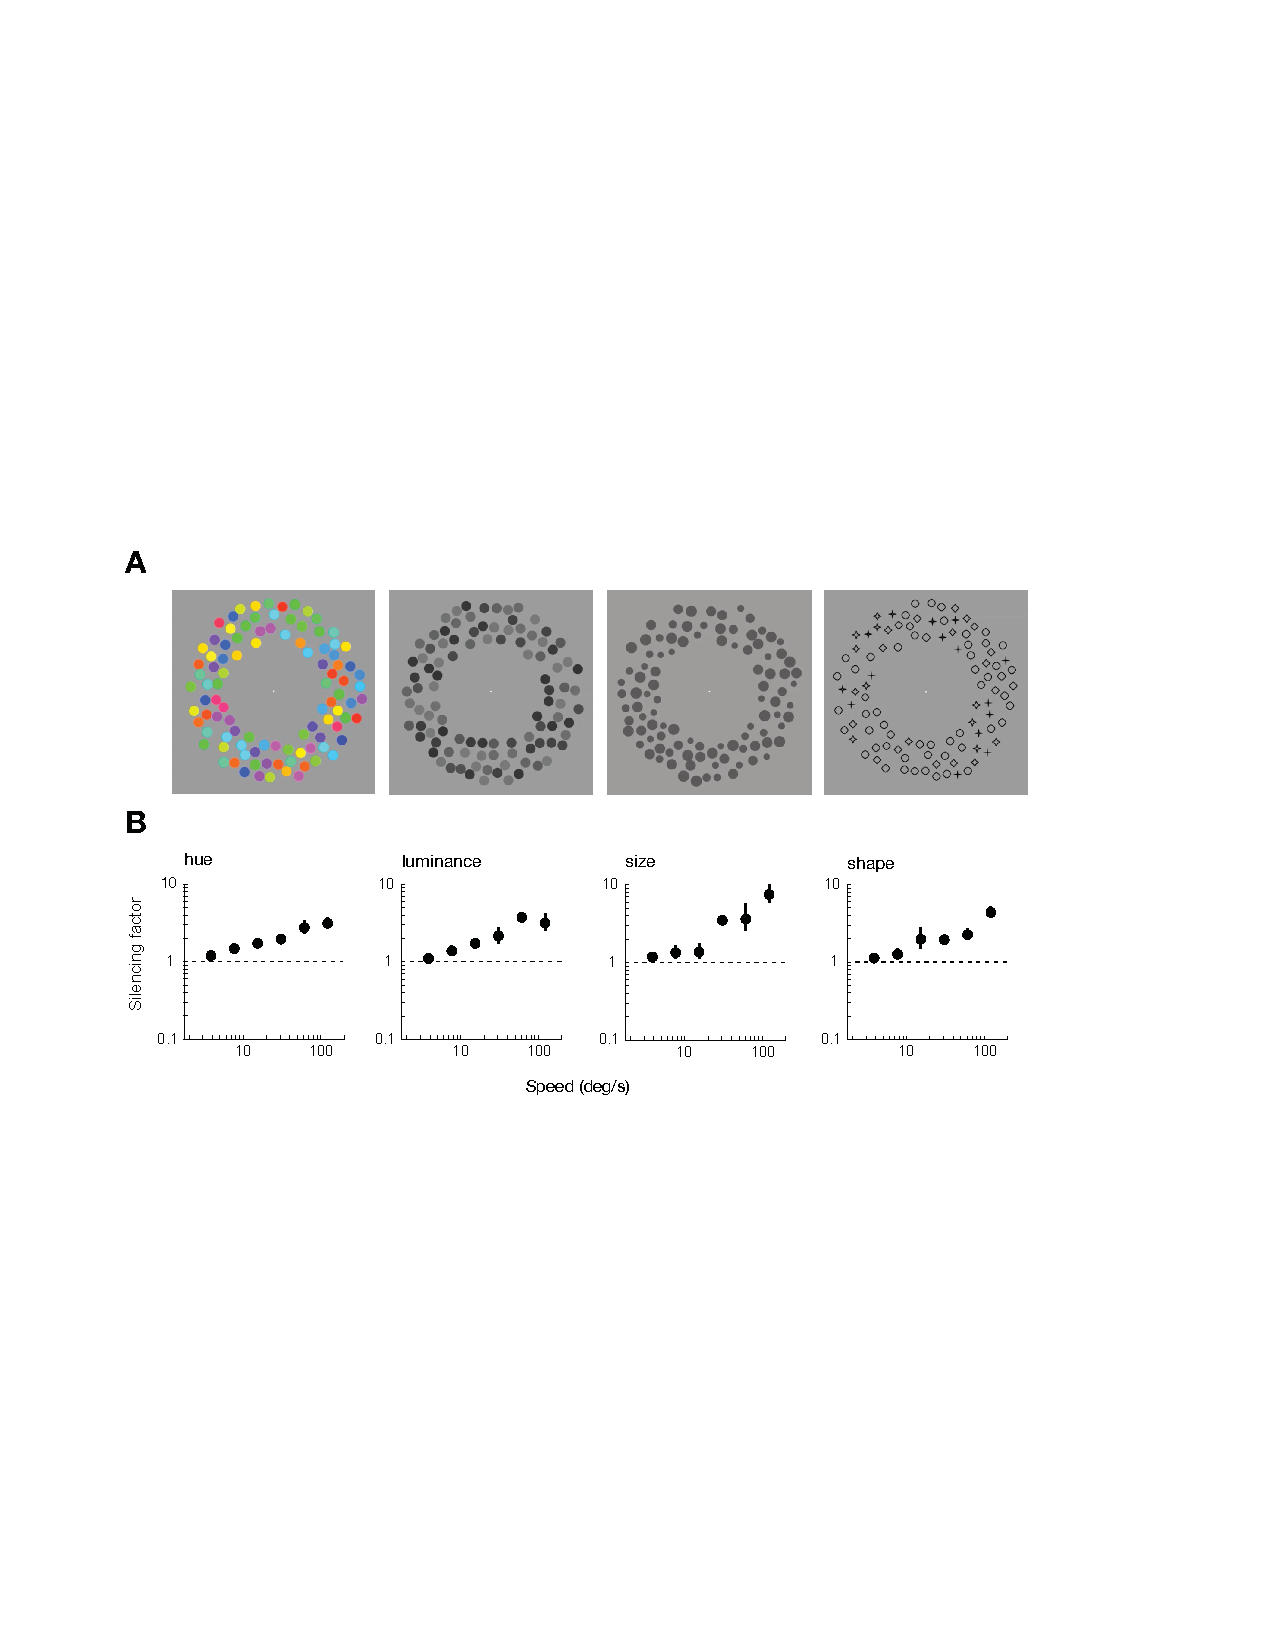
\includegraphics[width=\textwidth]{figures/fig1}
%\caption[Short figure name.]{This is a figure that floats inline and here is its caption.
%\label{fig:myInlineFigure}}
%\end{figure}
